\chapter{Uncertainty budget}\label{ch:Uncertainty}
Measuring an hadronic cross section  in LArIAT translates into counting how many hadrons impinged on a slab of argon at a given energy and how many of those hadrons interacted at said energy. So, the key questions here are:
\begin{itemize}
\item[]a) how well do we know the kinetic energy at each point of the tracking? %(Incident Kinetic Energy bins)
\item[]b) how well do we know when the tracking stops? %(Interacting Kinetic Energy bin)
\item[]c) are there any systematic shifts?
\end{itemize}

In order to answer this question, will discuss first a simple scenario  were our beam is 100\% made of pions which arrive as primaries in the TPC (no decay in the beam and no inelastic interaction before the TPC front face). We will then add a layer of complexity by discussing how we handle beamline contamination.

\section{Pure beam of pions}
Assuming a beam of pure pions gets to the TPC, let us explicit some of the variables in the kinetic energy equation \ref{eq:KEj}  to point out the important quantities in the uncertainty budget,

\begin{align}
 E_{j}^{kin} &=  E_{Beam}^{kin}  - E_{loss} - \sum_{i < j} \frac {dE_i}{dx_i}*dx_i\\
                  &=  \sqrt{p^2_{Beam} - m^2_{Beam}} - m_{Beam} - E_{loss} - \sum_{i < j} \frac {dE_i}{dx_i}*dx_i.
\end{align}

\subsection{Uncertainty on $E_{Beam}^{kin}$}
Let us start by discussing the uncertainty on $E_{Beam}^{kin}$. Since we are assuming a beam of pions, the uncertainty on the value of mass of the pion ($m_{Beam}$) as given by the pdg is irrelevant compared to the momentum uncertainties, thus $\delta E_{Beam}^{kin} = \delta p_{Beam}^{kin}$. 
We estimate the momentum uncertainty as follows.

\textcolor{blue}{  
We estimate the uncertainty on a 4-point track. In case of 3-points track, we add an additional 2\% coming from Greg's study. 
Uncertainty on a 4-point track:
\begin{itemize}
\item[-]  Alignment surveys. 1mm misalignment translates to 3\% in overall
\item[-] Doug study dp/p = ~2\% based on field map (docdb 1710)
\item[-] Minerva test beam paper
\end{itemize}
}

\subsection{Uncertainty on $E_{loss}$}
We estimate the uncertainty on the energy loss between the beamline momentum measurement and the TPC, $E_{loss}$, using the DDMC pion sample. We shoot pions from WC4 with the same momentum distribution as in the beamline data and plot the true $E_{loss}$ for that sample. The width of the $E_{loss}$ distribution is the $\delta E_{loss}$.

\textcolor{blue}{ TO DO HERE: make sure we have the geometry right, cause otherwise this correction is meaningless.  With this method, so far we get a mean ~40 MeV, but uncertainty ~7MeV. 
The trajectory method does not improve uncertainty, why? It's a mystery I don't think we should solve before June :) .
Back of the envelope material budget calculation:}
\begin{table}[h!]
\centering
\caption{Back of the envelope calculation}
\label{my-label}
\begin{tabular}{|l|l|l|l|}
\hline
dEdx for MIP, MPV {[}MeV cm$^2$/gr{]} & density {[}g/cm$^3${]} & width {[}cm{]} & E$_{loss}$ {[}MeV{]} \\ \hline
1.6                                                 & 1.7 (G10)                            & 1.3            & 3.5                   \\
1.6                                                 & 1.4 (LAr)                            & 1.77           & 4.0                   \\
1.6                                                 & 7.7 (S.S.)                           & 0.23           & 2.8                   \\
1.6                                                 & 4.5 (Ti)                             & 0.04           & 0.3                   \\ 
1.6                                                 & 1.03 (Plastic Sci)                   & 1.1            & 1.8                   \\ \hline
Total                                               &                                      &                & 12.4                  \\ \hline
\end{tabular}
\end{table}


\textcolor{blue}{Event taking into account a 3 degree bent, we get 12.41 MeV, which is quite far from 40 MeV... something smells here ;)}

\subsection{Uncertainty on dE/dx and pitch}
We obtain the uncertainty on dE/dx and track pitch by comparing the dE/dx and pitch distributions in data and MC.
\textcolor{blue}{ Currently, MPV MC = 1.70 and MPV DATA = 1.72 MeV/cm (~3\% higher).
TO DO HERE: calculate Argon density from mid-RTD temperature. Compare this  density with MC Argon density. 
Density change  affects dE/dx (in MeV/cm!). Try changing MC density up to ``real one" and see if dEdX agrees between DATA and MC}


\subsection{Uncertainty on track end, aka efficiency correction}
From the MC, we obtain an efficiency correction on the interacting and incident distributions separately. This is done by comparing the MC reconstructed with the true MC deposition on an event by event basis.
This correction is applied bin by bin on the data interacting and incident distributions.
The better our tracking, the smaller this efficiency correction will be. So, step number one is improving the tracking.
\textcolor{blue}{Need to talk to Bruce about this.}
\textcolor{blue}{ I don't understand the angle cut that Dave Schmitz and Jon Paley were so vocal about.}

Now, the key question remains: does the tracking behave in the same way in data and MC? 
We can compare some key plots between reconstructed data and MC which gives us confidence this is true: the track pitch, the tracks straightness and the goodness of fit in data and MC. \textcolor{blue}{ Does such a variable as ``goodness of fit" exists in the tracking? We should ask Bruce.}

\section{Handling beamline contamination}
What is the beamline contamination? We define beamline contamination every TPC track matched to the WC track which is not a primary pion. There are 4 different types of beamline contaminations:
\begin{itemize}
\item[]1) electrons,
\item[]2) muons,
\item[]3) secondaries from pion events,
\item[]4) matched pile up events.
\end{itemize}

So, how do we handle this contamination?

The first step is to estimate what percentage of events used in the cross section calculation is not a primary pion.  
We estimate the percentage of electrons and muons in the beam via the beamline MC\footnote{Since the beamline composition is a function of the magnet settings, we simulate separately events for magnet current of -60A and -100A. 
We calculate the electron to pion and muon to pion ratio on the whole sample as the weighted sum of the corresponding ratio in the two current settings, 
\begin{equation}
\frac{N_e}{N_\pi}_{Data} = w_{60A}\frac{N_e}{N_\pi}_{60A}  + w_{100A}\frac{N_e}{N_\pi}_{100A},
\end{equation}
\begin{equation}
\frac{N_\mu}{N_\pi}_{Data} = w_{60A}\frac{N_\mu}{N_\pi}_{60A}  + w_{100A}\frac{N_\mu}{N_\pi}_{100A},
\end{equation}
where the weights $w_{60A}$ and $w_{100A}$ are the percentage of events in the corresponding magnet configuration passing the mass selection in data. }.
Once the beam composition is know,  we simulate the electrons, muons and pions with the DDMC and we subject the three samples to the same selection chain (WC2TPC match, shower filter, pile up filter, etc...). The percentage of electrons and muons surviving the selection chain is the  electron and muon contamination in the pion cross section sample.
The percentage of secondaries is given in the MC by the number of matched WC2TPC tracks which are not flagged as primary by Geant4.
We estimate the last type of contamination, the ``matched pile up" events, to be a negligible fraction, because of the definition of the WC2TPC match: we deem the probability of a single match with a halo particle in the absence of a beamline particle\footnote{ Events with multiple WC2TPC matches are always rejected.} extremely small.


Once we estimate the contaminants to primary pion ratio, the next step is subtracting their contribution from data for each type of contaminant independently. The contaminant samples are reconstructed and the corresponding interacting and incident histograms are produced. We then perform a bin by bin subtraction in the data interacting and incident histograms separately. A graphical rendering of this procedure is shown in Fig \ref{fig:backgroundSubtraction}
Once the data is background subtracted, we apply the correction laid out in the previous section.
\textcolor{blue}{How do we account for the error in the contamination subtraction? We change the electron/pion and muon/pion ratio and we see how much difference we get?}

\begin{figure}
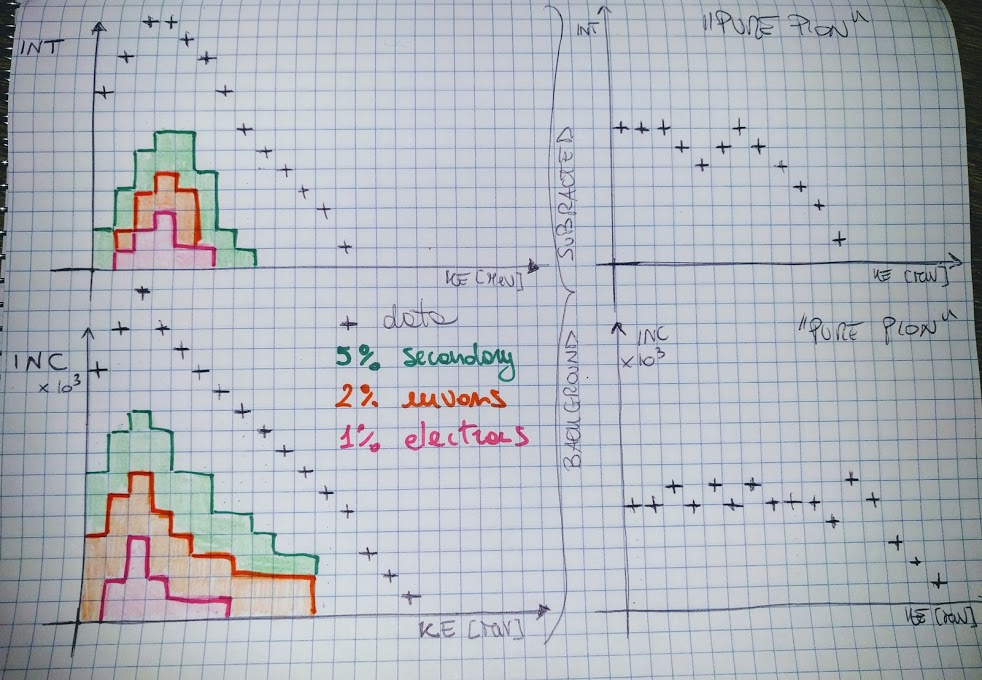
\includegraphics[width=\textwidth,height=\textheight,keepaspectratio]{Chapter-8/Images/FakePlot.jpg}
\label{fig:backgroundSubtraction}
\caption{A graphical rendering of the beamline contamination background subtraction. The contribution of the contaminants is shown in green for the secondaries, in orange for the muons and in pink for electrons. The colored plots are coming from the MC and are staggered. The percentages shown in the legend are the percentages of contaminants over the total number of events  passing the selection chain. We actually expect way less contamination.}
\end{figure}



